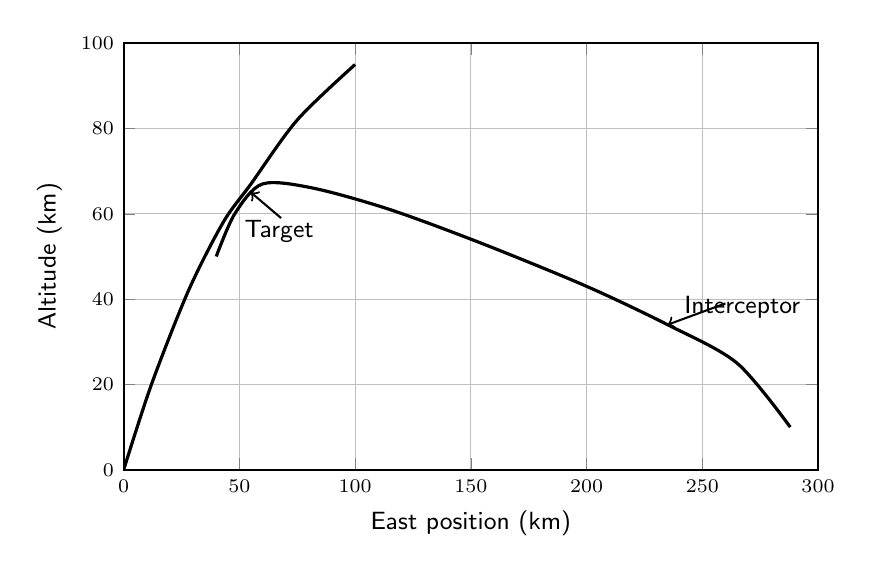
\begin{tikzpicture}
\begin{axis}[
  width=10.4cm,height=7.0cm,
  xmin=0,xmax=300,ymin=0,ymax=100,
  xtick={0,50,100,150,200,250,300},
  ytick={0,20,40,60,80,100},
  grid=major,
  axis line style={line width=0.8pt},
  tick label style={font=\scriptsize},
  label style={font=\sffamily\small},
  xlabel={East position (km)},ylabel={Altitude (km)},
]
  \addplot[line width=1.15pt,smooth] coordinates {(0,0) (12,20) (28,42) (43,58) (55,67) (75,82) (100,95)};
  \addplot[line width=1.15pt,smooth] coordinates {(40,50) (48,60) (60,67) (82,66) (115,61) (155,53) (200,43) (235,34) (265,25) (288,10)};
  \node[font=\sffamily\small,anchor=west] at (axis cs:48,56) {Target};
  \draw[->,line width=0.75pt] (axis cs:68,59)--(axis cs:55,65);
  \node[font=\sffamily\small,anchor=west] at (axis cs:238,38) {Interceptor};
  \draw[->,line width=0.75pt] (axis cs:260,39)--(axis cs:235,34);
\end{axis}
\end{tikzpicture}
